\renewcommand\chapname{Wiki/CMS approach, Language Archiving Technology, and TEI}	
\renewcommand\longchapname{Digital Grammars: Integrating the Wiki/CMS approach with Language Archiving Technology   and TEI}
\renewcommand\shortauthor{Sebastian Drude}
\renewcommand\longauthor{Sebastian Drude\\ Max Planck Institute for Psycholinguistics}
\chapter*{\longchapname}
\chapterauthor{\longauthor}
\mytoc{}
 
\begin{abstract}
 Although intrinsically closely related to the new field of language documentation, grammaticography is still mostly oriented to the book model, usually falling short of making use of related digital resources and hypertext functionalities. In this contribution, we show and discuss possible or easily achievable advances that can built on top of existing technology such as Language Archiving Technology as developed at The Language Archive at the MPI-PL: Exemplars and examples can be found in multimedia corpora of natural speech events annotated with ELAN and visualized with ANNEX, words and word forms can be linked to lexical entries in LEXUS online-databases, and the precise meaning of theoretical concepts can be given in ISOcat entries or related terminological databases. Independently from LAT, Wiki-technology provides online collaboration and version control and opens even the possibility to address different audiences in related sets of pages, but also poses challenges for the overall didactic structure of a descriptive work. As one of the formats, at least for export and exchange, the XML-based TEI may provide a suitable framework, although many specialized tags would still have to be introduced and formatting and functionalities for these tags still has to be implemented. Generally, synchronization between different versions (e.g., on-line and off-line) poses the most intriguing difficulties, but the advantages (also in terms of Nordhoff's maxims) of hypertext grammars as proposed here are overwhelming.
\end{abstract}


\section{Introduction} \label{drude:sec:1}

In recent years, core linguistic disciplines such as language description and linguistic typology have been undergoing major methodological changes due to the rapidly developing digital opportunities and a new interest in the world's linguistic diversity, in particular in endangered languages. The emergence of the new field of language documentation \citep{Himmelmann1998,GippertEtAlEd2006} is both result of and driving force for this development which according to some has the potential for an ``empirical turn'' or even ``revolution'' of linguistics and the humanities \citep{Newman2008, Gippert2010,Whalen2004}.

Also computational linguistics (natural language processing) has started to work with data from small languages and to make contributions to language documentation (e.g. \citet{Bird2009}, \citet{BenderEtAl2010clislt}).

While more and more digital empirical data becomes available and used, scholarly work about languages, in particular grammars, is usually still published as paper-oriented texts, mostly as books, book chapters or articles. Connecting scientific texts with their empirical basis and generally with other related resources is still a desideratum; much of the envisaged ``virtual research environments'' still has to be developed.\footnote{\citet{Thieberger2006} presented pioneering work akin to DGs as proposed here. See also \citet{Thieberger2009}.}

The present contribution discusses technology and proposals for an authoring and reading environment for ``digital grammars'', highlighting the potential role of Language Archiving Technology which does not yet include or develop such an environment.\thanks{The 
 ideas put forward in this contribution have been developed and refined in many discussions with several colleagues, all of which I would like to thank for their valuable input. Among these are Anthony Aristar, Helen Aristar-Dry, Jost Gippert, Jeff Good, Alexander Mehler, Sebastian Nordhoff, Laurent Romary, Albert Russel, Nick Thieberger, Dieter Van Uytvanck, Huib Verwey, Menzo Windhouwer, and Peter Wittenburg. It was not possible in each case to recognize a particular contribution by a specific person, for which I apologize. Of course the responsibility for shortcomings is mine alone.} Many of the aspects discussed here exist (or have been proposed) already individually; the goal of this contribution is primarily to provide a survey of the relevant technology, existing or in development, and to propose to combine certain specific aspects and solutions. To the best of my knowledge, several individual features and their combination are proposed here for the first time. The development of a technological solution that includes all of the features suggested here will need at least a medium-sized project with more than one developer and ideally involving several institutions; a project which still needs to find funding. But even at this planning stage the ideas and views put forward in this contribution should serve to stimulate the debate and to gather a group of interested people and institutions.

The focus and general approach of this paper are akin to work by Good, Nordhoff and others.\footnote{See, 
 in particular, \citet{Good2004,GoodEtAl2010,Nordhoff2007tgasg,Nordhoff2007gwea,Nordhoff2007ggwg}.
} 
\citet{Nordhoff2008} introduced a number of (possibly conflicting) values that may govern the development of such a system, and for each value one or several ``maxims'' (roughly, design features) that honour the value. 
Nordhoff refrains [298] from endorsing any of them, but most are indeed pertinent and should be taken into account in one way or another. Wherever appropriate, I will refer to N's values and maxims, presupposing his discussion.\footnote{I 
 usually refer just to the maxims by ``N[ordhoff]'s maxim \#'' without citing \citet{Nordhoff2008} in every instance. A
 list of these maxims is given in the appendix of this volume.
}

Slightly differently from Good and Nordhoff, I here use the term ``grammar'' as representative not only for comprehensive language descriptions but generally for linguistic work based on primary linguistic data (i.e., mostly on recorded speech events as typically obtained in field research), including typological/comparative or more specific descriptive studies. By ``digital'' I refer not only to the distribution form but imply the broad use of information technology and functionalities such as hypertext links inside and outside the document.

\section{Digital (Hypertext) Grammars}  \label{drude:sec:2}
The possibilities of developing grammars as digital (hypertext) documents has been put forward since the late 1990s \citep{Zaefferer1998}, and recently the topic of general and also of digital ``grammaticography'' has gained attention \citep{AmekaEtAlEd2006,Lehmann2004dog,Lehmann2004fg,PayneEtAlEd2007}.\footnote{Particularly 
 relevant was the \textit{Conference on Electronic Grammaticography} organized by Nordhoff at the 2\textsuperscript{nd} International Congress on Language Documentation and Conservation in February 2011.
} 
Nevertheless, there have been only few and partial attempts at developing a digital infrastructure for linguistic research which includes interlinking the linguistic scholarly texts with spoken samples of language use and other resources.

The major special feature of the digital medium is the possibility to \textit{add functionalities} to pages or individual elements of a text. In the case of classical hypertexts, for instance, \textit{links} connect to other parts of the same text or even to other documents, locally or in the World Wide Web. Further functionalities are for instance database queries or playback of multimedia resources. In this way, a text can be embedded into an environment of related external digital resources.

For the purposes of digital grammars as envisaged here, in agreement with \citet{Good2004}, I consider the following complementary digital external resources to be most relevant:

\begin{enumerate}
\item \label{bkm:Ref296272363} a language archive with a corpus of annotated recordings of naturalistic and elicited speech events (Good's  ``texts'');
\item \label{bkm:Ref296272365} a dictionary/lexical database with lexicographic descriptions of individual words and similar units  (Good's  ``lexicon''); 
\item \label{bkm:Ref296272357} a resource where the underlying concepts and the meaning of the applied terms are explained and made explicit  (Good's  ``ontologies'').
\end{enumerate}

These external resources (which can be respectively abbreviated as ``text database'', ``lexical database'' and ``terminological database'') are discussed in section~ in more detail.

Based on these, I propose the following features and functionalities as crucial for a digital grammar (DG):

\begin{enumerate}
\item The DG is, or can be rendered as, a set of organized and interlinked hypertext pages (see Section \ref{drude:sec:4}).
\item \label{bkm:Ref296267835}Recordings of exemplars  (didactic linguistic examples)\footnote{I 
 follow here the terminology of \citet{Good2004}.
} can be replayed together with their annotation.
\item More relevant examples for specific phenomena can be searched in and retrieved from the text database and/or lexical database.
\item \label{bkm:Ref296267849}Individual lexical entries for individual words cited in the DG can be looked up in the lexical database.
\item \label{bkm:Ref296267853}The meaning of technical terms used in the DG can be looked up in the terminological database.
\end{enumerate}

The relations to the three external resources (a), (b), and (c) can be illustrated as in Figure \ref{drude:fig:1}. The main relevant functionalities are represented by arrows: (e) green, (g) yellow, and (h) blue.


\begin{figure}
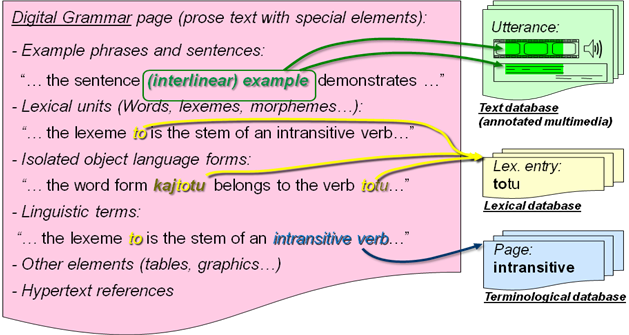
\includegraphics[width=\textwidth]{\imgpath/Drude-img1.png}
\caption{Principal external relations of a DG}
\label{drude:fig:1}
\end{figure}

\section{Language Archiving Technology}  \label{drude:sec:3}
The three external resources proposed to interact with a DG are not new by themselves. In particular, as to the text database, the construction of comprehensive language corpora with annotated recordings of speech events is the very core of language documentation activities as practiced by dozens or even hundreds of projects carried out worldwide in the last 10 years or so.

Digital lexical databases are probably the earliest language resources created with computers in a field research context. Terminological databases, in turn, are better known in the area of natural language processing, for instance for (automatic or manual) translation. They could add value, however, to grammars, which often have been written on two different levels: in many instances, (1)~a specific theoretical conception of a certain domain is explained and the analytical concepts are introduced before [or while] (2)~the specific terminology is applied in describing the language (data) at hand.\footnote{This 
 holds in particular for grammars which are explicitly formulated in a specific theoretical framework. If their terminology is not carefully explained, the grammar runs the risk to be opaque and incomprehensible to anyone not familiar with that particular approach. But also grammars that claim to be ``theory neutral'', mostly using widely used linguistic terms, need to make the exact meaning of the employed analytical concepts explicit because the ``basic'' linguistic terms often have varying or vague meanings.
}
The digital technology allows to keep these two levels apart, so that the DG can focus on the description and analysis, directly employing the terms which are defined and explained in an external terminological database.

One major challenge for all three external resources is: in which form and based on which technology can they be made available for an optimal (in particular, lasting) interaction with the DG? Several solutions may exist for each of them. For instance, there are a few central and several regional language archives, possibly with different standards with respect to file formats and metadata.

Language Archiving Technology (LAT) is a group of interrelated software tools which aims at providing coherent and lasting solutions for the challenges concerning all three external resources identified above. It is developed mainly at the \textit{Max-Planck-Institut f\"ur Psycholinguistik} in Nijmegen (MPI-PL) by what is now ``The Language Archive''. This recently founded unit (earlier the technical group at MPI-PL) is the technological centre of the program ``documenting endangered languages'' (DOBES, funded by the Volkswagen foundation), which was one major reason for developing LAT.

The LAT  suite is comprised of a well-known tool for annotating audio and video language use data, ELAN \citep{WittenburgEtAl2006}, an online service for creating and accessing lexical resources \citep[cf.~LEXUS][]{RingersmaEtAl2007}, and tools for metadata-based access to resources using the IMDI metadata standard \citep{IMDITeam2003}.\footnote{The 
 IMDI-standard is now being superseded by a new CMDI standard developed in CLARIN, the current pan-European initiative to create, coordinate and make language resources and technology widely available and readily useable, one of the core pillars of developing the ``Digital Humanities'' \citet{SchreibmanEtAl2008}.
} 
Metadata can be created with a dedicated editor and now with the ARBIL tool \citep{Withers2009}, and the archive can be browsed and accessed with the IMDI-browser. With the LAMUS tool \citep{Broeder2011}, authorized users can upload resources to the archive while consistency checks are performed. User and access administration is done with the AMS tool \citep{AMS-II}. The resources can be explored online with tools such as ANNEX/TROVA (for multimedia with annotation created with ELAN), LEXUS (for lexical data) and IMEX (for images). Last but not least, the central ISOcat data category registry \citep{Kemps-SnijdersEtAl2009} allows defining concepts to which all resources can refer so that different terminologies can be made interoperable.

Most importantly, the language archive has been built with sustainability and long-term-preservation in mind. It is one of the very few archives which have an institutional commitment (for at least 50 years). It uses persistent identifiers (PIDs, cf.~CLARIN) to ensure that objects can be cited and recovered even if the infrastructure and location of resources changes (cf. N's maxim~24). Several local and regional archives worldwide are adopting the LAT infrastructure. Even if the technology is bound to change, new technology will be backwards compatible and many other independent developments will at least be interoperable with LAT and its successors. 

Crucially, no module for developing grammars (in the broader sense, empirical linguistic work based on speech data) is part of the LAT suite so far, although the basis for building such a platform and integrating it into the existing technology exists. Therefore, LAT is an ideal environment for the development of a digital grammar authoring environment, which is one of the most important points of this contribution. In the next paragraphs, I will discuss the LAT solutions for the three external resources one by one.

The first external resource identified above, the text database for a digital grammar (DG), can be precisely a LAT language archive with IMDI sessions containing ELAN (\texttt{.eaf}) files and the multimedia files they annotate (see figures~2 and~3). An archived ELAN file can be referenced to by its PID, and the ANNEX tool can be used to display and play specific parts of a recording, for instance one sentence of a text, together with its annotation. This allows implementing N's (2008) maxims 1~\&~2 (regarding accountability): each example/exemplar can be traced back to a real utterance. The context of the examples is also immediately accessible in an ELAN file (N's maxim~4). Using searches (e.g., with the LAT online tool TROVA), more examples can be found in the corpus (the text database) and also be displayed in ANNEX (N's maxim~3).


\begin{figure}
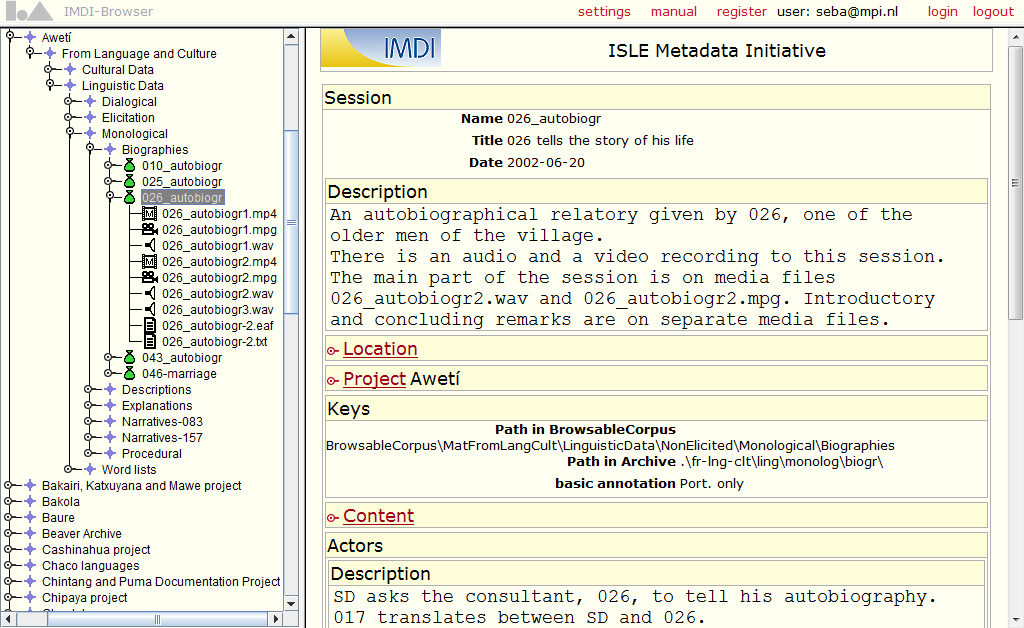
\includegraphics[width=\textwidth]{\imgpath/Drude-img2.jpg}
\caption{ A LAT based language archive with an IMDI session }
 \end{figure}



\begin{figure}
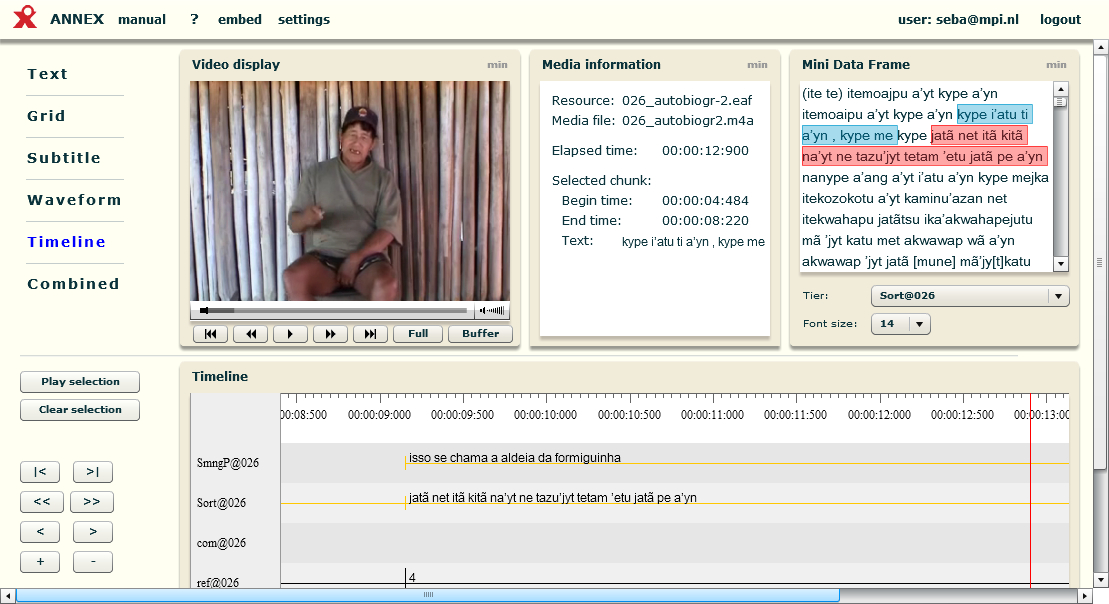
\includegraphics[width=\textwidth]{\imgpath/Drude-img3.jpg}
 \caption{An ELAN annotation file displayed in ANNEX}
\end{figure}

Creating and exploring lexical databases (LDs, the second external resource of DGs) is the very purpose of the LEXUS tool. Currently many LDs in LEXUS have been imported from other tools such as toolbox (formerly shoebox), and interchange with other lexical database tools will continue to play an important role.\footnote{The 
 ongoing RELISH project at the MPI-NL, University Frankfurt and Institute for Language Information and Technology at the East Michigan University aims at making different lexical resources, in particular LEXUS (LMF) databases and LIFT-compatible databases interoperable.
}
Still, differently from Toolbox, LexiquePro, FLEX and other lexical tools, LEXUS relies on the ISO standard LMF \citep{FrancopouloEtAl2007}; see also \citet{RingersmaEtAl2010} for LDs and is designed to provide full multimedia support.\footnote{Very 
 recently, the LEXUS tool has undergone a complete re-implementation, and more major improvements regarding user interface and functionalities are foreseen for the next future. For instance, it is planned to integrate LEXUS with ELAN so that semi-automatic glossing of sentences and texts based on lexical data (at least including functionalities known from Toolbox or FLEX) becomes possible.
} 
Although work on a stand-alone version is making progress, LEXUS is fundamentally web-based, and uses also PIDs so that integration with other tools is straightforward. 


\begin{figure}
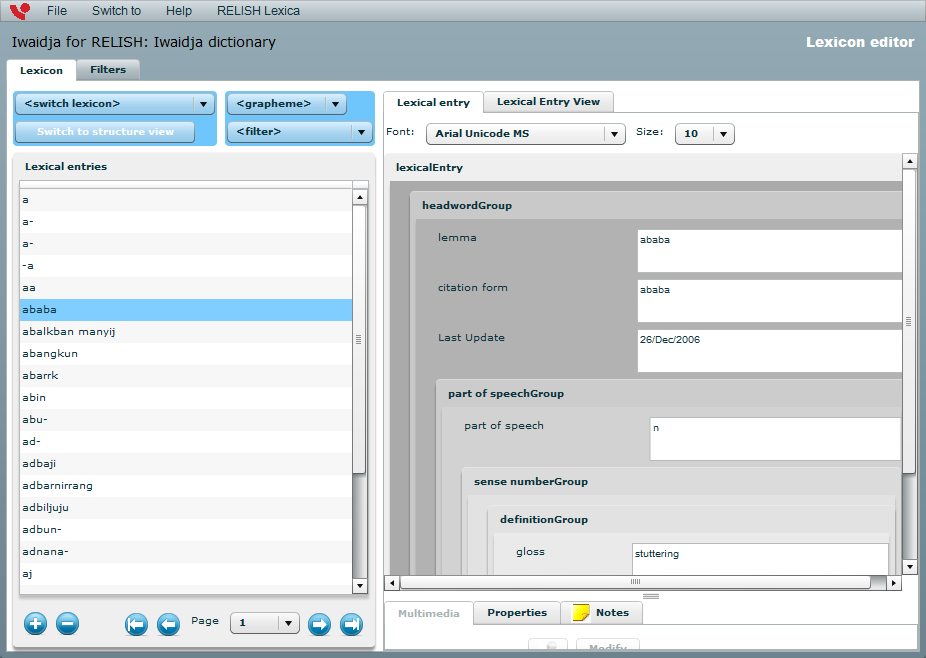
\includegraphics[width=\textwidth]{\imgpath/Drude-img4.png}
\caption{A LEXUS lexicon}
\end{figure}
 
Finally, the purpose of the more recent ISOcat data category registry is to be a central location where definitions of terms for all areas of linguistics and language technology can be provided so that documents and other resources can refer to them. By defining relations between different entries (the ``substantive'' in one framework can be very close to equivalent to the ``noun'' in another framework), language resources are prepared for the semantic web \citep{W3C2011,GoodEtAl2010}. As such, ISOcat can be a central reference or starting point for the terminological database as proposed here. This holds for Good's 2004 ``general'', ``subcommunity'' and ``local ontologies'' alike, which in ISOcat can be distinguished by creating ``collections'' of terms. The GOLD \citep{FarrarEtAl2003} terms have been included in ISOcat by the RELISH  project and are available as one such selection.

\begin{figure}
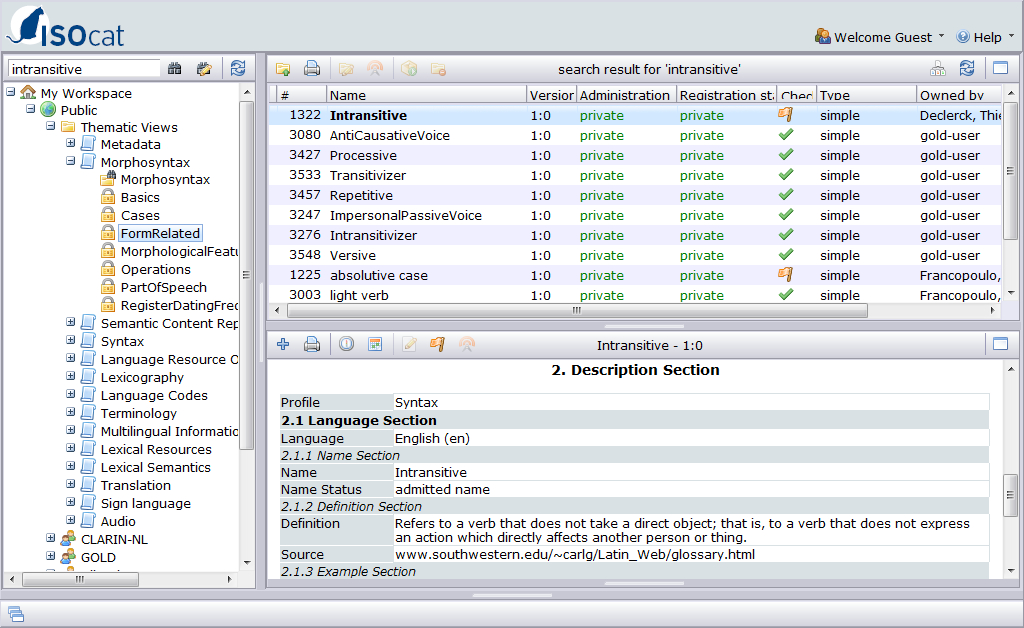
\includegraphics[width=\textwidth]{\imgpath/Drude-img5.jpg}
\caption{The ISOcat category registry}
\end{figure}

Possibly, for the purposes of descriptive linguistics, at least some frameworks will need a more integrated terminological resource with richer explanations than the small text-only technical definitions that are usually given in ISOcat. We propose that such frameworks build their own reference system, for instance in the form of a Wiki, but use ISOcat as a point of reference (where short definitions should be provided). But also less theory-specific descriptions should still link their terms to a corresponding ISOcat entry (which generally will exist, at least for most general terms) in order to guarantee interoperability with other resources. The other LAT tools are all prepared to interoperate with ISOcat, so that this appears to be an ideal starting point for the third external resource, the terminological database (for any kind of online documents involving linguistic terminology).

\section{The Wiki/Content Management System approach} \label{drude:sec:4}

As stated in (d) above, a DG should be, or should be able to be rendered as, a set of organized and interlinked hypertext pages. Certainly, however, grammarians, descriptive linguists or typologists are rarely prepared and willing to edit hypertext pages by hand;\footnote{But 
 see the work by Lehmann, presented at the Colloquium on Grammaticography at ICLDC 2.} probably only a minority is regularly using semi-logical mark-up like (La)TeX \citep{Knuth1992}.

Nowadays, websites can be created and edited in Content Management Systems (CMSs) where the content can be entered in an environment similar to better known office software. In particular, the more specialized Wiki-technology is now widely known and used (in rough technical terms, the functionalities of Wikis are a subset of those of CMSs). \citet{Nordhoff2007tgasg,Nordhoff2007gwea,Nordhoff2007ggwg}, elaborating on proposals by \citet{Weber2006}, has proposed and developed ``Galoes'', a Wiki-based online grammar authoring environment.

Indeed, a CMS-based solution has several major advantages, among these:

\begin{enumerate}
\item it is independently existing software, so it has not to be developed and maintained or updated by the developers of the DG system;
\item it usually has version control, which allows inspection of the development of the analysis over time, and going back to previous versions (cf.~N's maxim~7); 
\item it allows collaboration of different users (at different places), and individual contributions are automatically related to their respective authors (N's maxims~11~\& 12 on collaboration); 
\item user-management (usually included) permits to control rights of editing etc. for different kinds of users;
\item it allows for full-text searches, generating an index or dynamic thematic listings of pages (which can be ``tagged'' for this purpose), etc. (N's maxim~15).
\end{enumerate}
On the other hand, there are several major challenges for existing CMS or Wiki systems:

\begin{enumerate}
\item \label{bkm:Ref297464324}most additional functionalities identified in section~2 have to be implemented to ensure integration with the external resources and generally with other (e.g., LAT) tools;
\item \label{bkm:Ref297464521}the Wiki-syntax or display-oriented formatting which usually exists in CMSs is not sufficient for distinguishing the ontological status of the different special linguistic objects;\footnote{For 
 instance, marking an object-language entity with the display formatting ``italics'' does not distinguish between sentences, phrases, isolated word forms, lexemes, syllables etc., each of which may have different associated functionalities. Also, the display formatting may in fact change according to the theoretical framework or the degree of formality/the audience.}
\item \label{bkm:Ref297461869}in particular in a Wiki-like environment, the pages are basically unordered, which impedes a didactical linear arrangement in a sequence of chapters, sections and so forth.
\end{enumerate}

In order to allow solutions for first challenge (f), the CMS has to be extensible (preferably open source). It has been discussed in the previous section that the LAT tools (in particular by using PIDs) are prepared for integration and interaction. 
The second challenge (g) will be discussed in the next section. As to the last point (h) \citet{Nordhoff2008} advocates for nonlinear grammatical descriptions, although admitting that this approach creates difficulties for his maxim 20 (on a didactical presentation).\footnote{The 
 same holds, if less grievously so, for the maxim~21 on the ease of complete reading.
} 
I believe this maxim to be important for most scholarly work, even when using digital technology.

Therefore, I propose, at least as an option, a linear organization in units like parts, chapters, sections, etc. where each organizational unit is represented by one hypertext page; units higher in the hierarchy should contain automatically generated listings of links to their respective sub-units (in addition to an optional introduction or overview). Almost every page should have, then, a clearly defined ``previous'', ``next'' and ``upper'' page,\footnote{Such 
 a linear structure also is the easiest solution for the exhaustive perception problem for readers that which to read the complete description (albeit arguably a minority); cf.~N's maxim~21.
} 
although a reader can follow his own path when reading (in) a DG following links to related but distant pages or using tables of contents and indices (N's maxims~17 \&~18). Of course, the later introduction of an additional page in the middle of a unit, or the splitting of a page into two (while maintaining their place in the linear sequence of pages), or the rearrangement of the order and groupings of pages, are challenges that need to be solved without imposing the burden of manually updating links or unit numberings on the author.

\citet{Nordhoff2008} proposes to `tag' the pages according to their place in one or several standardized outline(s) for grammatical descriptions. This can indeed be useful for readers expecting or familiar with a certain structuring (N's maxim~19), but on the other hand, every linguist may have their own approach and every language may require its own best way to describe it (cf. N's maxim~10 on the author's creativity), so some authors may still choose an individual organization of their presentation. This holds much more for typological work or individual papers on specific aspects of a language. Still, `tagging' pages, e.g. for their relevance and quality (reliability), cf. N's maxims~22 \&~23, is an excellent proposal and easily implemented in a CMS-based DG system. 

Whether one adopts a (possibly standardized) hierarchical and linear organization or not, individual pages in a CMS allow the author to systematically address different groups of readers separately. This has the potential to overcome a notorious problem of grammars (it may occasionally also concern more specific and smaller linguistic scholarly texts): although the readers may be, for instance, laymen, general linguists (such as typologists), or colleagues that share highly specific theoretical assumptions and background (besides readers who may master different meta-languages, cf.~N's maxim~25), there is often only one grammar which either tries to satisfy the different needs in one document (for example by extensive use of footnotes) or else which ignores the needs of one or several groups of potential readers.\footnote{This 
 problem concerns descriptive grammars and is different from the well-known distinction between descriptive and didactic grammars; the latter are a completely different type of text which usually needs a rather different organization.
}

A CMS may be set up so that an author can create and manage several individual hypertext pages that all discuss the same topic, albeit for different readers. The organization into different ``layers'' would be orthogonal to the linear and hierarchical organization, as is shown in~ Figure 6. In this way, a reader could choose a default layer so that the links usually point to respective pages (if they exist) of that layer. For a given chapter or section the reader still may choose to read another alternative version with, e.g., more or less detail.


\begin{figure}
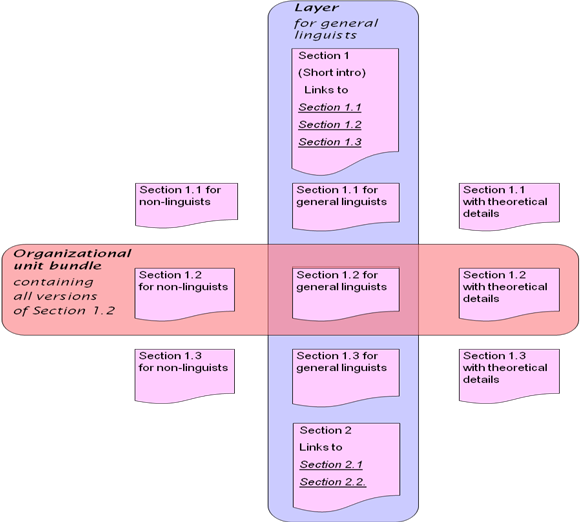
\includegraphics[width=\textwidth]{\imgpath/Drude-img6.png}
\caption{Organization in layers and organizational units (detail)}
\label{bkm:Ref299295833}
\end{figure}

It has been suggested by Nordhoff (maxim~9) that templates be provided by the system and applied by the authors of a DG in order to ease the creation of new pages with grammatical information \citep{Blacktv}. This might be useful for potentially highly uniform pages, such as pages that describe the form and function of individual morphemes in an agglutinative language (or functional particles in an isolating language), and can be implemented with a CMS or Wiki environment. However, I believe that such a formalized approach would be appropriate for only some parts of a comprehensive language description, and even less useful for more specific smaller work (see also N's maxim~10 on creativity, conflicting with his maxim~9).

In any case, most CMSs are configurable and flexible enough to allow for the authoring of linguistic scholarly work --- given the interconnected questions of the data format(s) and the corresponding suitable editing mechanism are solved.

\section{The Text Encoding Initiative} 
There are many different formats of and for digital document, and new formats are developed constantly while others become outdated and, after some years, difficult to access. This holds in particular for proprietary formats such as those generated by commercial office software, which is one major reason why a general authoring environment should rely on open and well documented and widely used formats. Such formats can be developed with XML, the extensible mark-up language, which promises to stay for a long time due to its flexibility to adapt the most different data types, and its wide and growing use.  Also, XML has the advantage of being readable both by humans and by machines, which opens possibilities for a later exploitation of DGs by other applications, and their integration into future larger ``virtual research environments''. This is one of the most promising paths that digital methods currently provide for linguistics \citep{BenderEtAl2010lingo}.

We therefore argue that a DG should have XML as one of its central data formats. We say ``one of'' and not ``the'', because any online authoring environment will certainly conceptually have to deal with several formats, at least some of which will be technically different one from another. For instance, there will be a format for display (e.g., HTML), a format for representation in the computer memory (the internal working format), a format for saving the work into digital file(s) for backup and/or exchange purposes, one for print-outs (e.g., PDF), perhaps another one for distribution in a stand-alone application, maybe still another one for entering and editing of the content by the user (such as Wiki-markup), and so forth. With XML as one basic format, some formats (such as HTML and PDF, perhaps via TeX) are possibly generated by the CMS without need for any further developments. The better structured the XML format, the more likely it is to take over several of these functions, relieving the burden of developing (often error-prone) routines for converting (parts of) the work from one format into another, some of them bi-directional, which are part of the challenges for the development of such an infrastructure. Also, based on XML, the data and description can later easily be used and manipulated for different purposes (cf also N's maxim~26). There are several CMSs that have an underlying XML format (e.g., Mapix, Baryshnikov, generally, see Content Management Directory).

Even if XML as one central format for the DG is granted, there are an infinite number of possibilities for the concrete elements and their structuring. Again, it is advisable to adhere, as far as possible, to existing standards. It seems to me that the standard being developed by the Text Encoding Initiative (TEI) is the most promising candidate, as it is widely recognized, particularly in the humanities, social sciences and linguistics (being used by almost 150 major and minor projects).\footnote{Another 
 candidate is the format used by the XLingPaper project, cf. \citet{Black2009,Black2010,Blacktv,SimonsEtAl2009}. Compatibility and interoperability will have to be carefully checked.
} 
There already exist first attempts at integrating TEI-XML in CMSs \citep{Schlitz2010}.

The TEI guidelines \citep{TEIConsortium2009} specify encoding methods for machine-readable texts, making concrete proposals for XML elements, attributes and their use and arrangement. XML can be the basic format for several purposes, in particular publishing \citep{ReedEtAl2009}. There are specific parts of the TEI guidelines that deal with entities relevant for the linguistic analysis.\footnote{In 
 particular, Section 17.1. ``Linguistic Segment Categories'', but also parts of chapter~8 ``Transcriptions of Speech'' and chapter~9 ``Dictionaries''.
} 
Still, there are potentially many entities which are specific to linguistic descriptions (in particular, interlinear text\footnote{For 
 explorative studies, see \citet{BowEtAl2003tgmilt,BowEtAl2003a4lmilt,HughesEtAl2004}. Also \citet{PalmerEtAl2007} propose a dedicated XML representation of interlinear text. The DG environment should build on this and similar previous work.
}). 
It seems advisable to add to the TEI guidelines a chapter or sections with elements for the specific needs for linguistic description, and there is an interest by members of the TEI consortium in adding this (Laurent Romary, p.c.).

On the other hand, the linguistic terminology varies among linguists and frameworks, and at least for certain parts of the terms applied in a language description this may well always be the case,\footnote{This 
 corresponds to Good's 2004 ``subcommunity'' and ``local ontologies''.
} despite the recent attempts at proposing a basic or universal common set (e.g. by GOLD [see references] or Dixon's ``basic linguistic theory'', cf. \citet{Dixon2010}). Therefore, for each DG the applied elements should be extensible beyond those foreseen by even a dedicated TEI module (cf. N's maxim~10 on creativity). Also, all elements should be configurable with respect to the following properties:

\begin{enumerate}
\item display/formatting (font properties, possible ontological distinctions), which may vary for different layers directed to different audiences (cf. N's maxim~8);
\item primary associated functionality (usually accessible by mouse-clicking on the item);
\item possible additional secondary associated functionalities (possibly accessible by a context menu or similar). 
\end{enumerate}

For illustration, three types of entities are probably referred to in any grammar, and would represent dedicated XML elements with the properties exemplified in Table \ref{drude:tab:1}.\footnote{Note 
 that the ontological type ``syntactic unit'' aims at arbitrary (e.g., inline) quotations of object language syntactic units. The ``see interlinear glosses'' function does not render interlinear text exemplars superfluous; these would continue to be the main type of example which should be displayed as such right away by default.
} 
Similar units and possibly further associated functionalities are needed for many other entity types on the phonetic, phonological, morphological, syntactic and semantic levels of linguistic description.

\begin{sidewaystable}
\begin{tabular}{p{2.5cm}p{4.5cm}p{3cm}p{2.5cm}p{4cm}}
\hline
  Linguistic/\newline ontological Type  &
  Tags and properties  &
  Formatting  &
  Main functionality  &
  Possible secondary functionalities\newline
 (tooltips and the like) \\\hline
  syntactic unit\newline
(sequence of words)  &
\texttt{<dg:Synt.Unit>\newline
 he goes \newline
</dg:Synt.Unit>}  &
 he goes 
 italics, roman &
  play \newline
media file &
see interlinear glosses 

see syntactic tree 

jump to lexical entries for individual words\\\hline
 individual word &
\texttt{<dg:Word>\newline
goes\newline
</dg:Word>}  &
  \textit{goes}
 italics, roman &
  see interlinear glosses for morphs &
jump to corresponding lexical entry (offering choice between homonyms)

play media file if exists\\\hline
  lexical word &
\texttt{<dg:Lex.Word  homonym.number=1>\newline
go\newline
</dg:Lex.Word>} &
 go\textsubscript{1}\textsuperscript{W}
 italics, roman, superscript W, subscript 1 &
 jump to lexical entry
 (taking homonyms into account) &
show meaning 

show word class

show occurrences\newline
of forms of the lexical word in texts\\\hline
  technical term &
\texttt{<dg:term\newline ISOcat="intransitive verb" PID="{\dots}"$>$\newline
intransitive\newline
</dg:term>} &
 intransitive 

 roman, upright\newline
(in formal context maybe sans serif) &
{show definition from ISOcat\newline
(or go to ISOcat entry)} &
go to explanation in theory-specific Wiki
go to page in grammar where this entity is discussed\\\hline
\end{tabular}
\caption{Linguistic entities, their XML representation and associated properties}
\label{drude:tab:1}
\end{sidewaystable}

These associated properties are part of the DG infrastructure and in principle independent of the TEI recommendation for elements and their attributes (or any other XML serialization), although some aspects of the functionalities may depend on the XML structure (such as the representation of homonym disambiguation by an attribute in the case of lexical words in Table \ref{drude:tab:1}).

\section{Versioning and publication} 
As many major reference works in the digital world, comprehensive language descriptions are not limited to static documents but they should be ``living'' --- often they need to be extended and revised as our knowledge about the language increases (cf. N's maxims 5 \& 6). This may hold, albeit in minor extent, also for smaller and more specific digital documents about particular aspects of one language, or for typological work which discusses data from different languages. A CMS solution promises to be an appropriate basis for the implementation of digital grammars as advocated here for the reasons discussed in Section \ref{drude:sec:4} (particularly, version control and management of multiple users). Still, ``living documents'' in general and digital grammars in particular present a number of challenges:

\begin{enumerate}
\item there should be only one central ``master'' instance of the DG which is maintained up to date;
\item other instances and copies, possibly in other formats (e.g., for distribution), should be derived from that master instance;
\item a certain version of the DG (e.g., a copy derived and distributed at a certain point of time) should be a citable reference (N's maxim~24);
\item the DG ideally should be editable when working with speakers ``in the field'' (N's maxim~13).
\end{enumerate}

Two main possible derived formats as suggested in (b) are:

\begin{enumerate}
\item book or paper versions for reading without digital equipment, e.g. in libraries and in the field (N's maxim~27);
\item stand-alone offline digital versions for distribution and reading on computers or similar devices (N's maxims~13 \&~16).
\end{enumerate}

The requirements for these two versions are radically different. The paper version needs a linear order of all pages, good formatting on all levels (individual XML elements, see last section, interlinear texts taken from the annotated corpus, sectioning, cross-references, etc.) and a consistent system of citing elements of the primary data (recordings) and their annotations in an appropriate form. Selected parts of the terminological and lexical databases and of annotated texts (without primary multimedia data) can be included. 

In addition, a stand-alone digital version should try to maintain most of the functionalities of the online DG, and therefore include relevant parts of the text database with their primary multimedia data. This not only needs large storage capacities, it also raises possibly complex issues of reorganizing and redirecting the many links so that they point to offline copies of the associated databases. These issues also turn up when it comes to citing specific parts of the DG and/or their associated databases; the specific version should be identified technically so that the relevant state of the work at the respective point of time can be retrieved although by default external links to a DG and its associated databases may prefer to point to always the current version (cf. N's maxim~6 on actuality).

Requirement (a) and generally principles of global availability suggest that the central master instance be online on some central server, as usually is the case of a CMS or Wiki. One master instance on a central server would also allow for automated backups (N's maxim~14 on safety) and (semi-)automatic curation, e.g. transformation to new formats when current formats become obsolete. Both issues are major challenges for the general goal of data sustainability \citep[cf.][]{BirdEtAl2003}.

However, this requirement conflicts with requirement (d) --- on many field sites there is no access to the internet. Allowing for editable offline instances of a DG posits even more complex problems of linking than in the case of offline distributions for exploring and reading. In particular, the need for synchronization of different versions (typically, an offline instance edited in the field with the central online instance) introduces many complex technical issues. Some may be addressable by using an appropriate XML format (see section~5) and established ``diff'', ``patch'' and versioning software (such as Apache Subversion or similar revision control systems). Others may require ``logging'' of changes and their ``replay'' on the central instance, in particular if changes involve the external databases or major rearrangements of the DG. Although the need for offline editing is obvious for use by field linguists, this feature certainly will take much more time than other aspects of the development of a DG.\footnote{This 
 can be seen by the development of the lexicon software LEXUS at the MPI/TLA: although a known demand since its beginning, the offline version of LEXUS is still in an experimental stage.}

\section{Conclusion}

The time seems ripe for the development of a general environment for digital grammars. Much of the necessary technology is available, in particular the technology for the primary external resources connected to a DG: text, lexical and terminological databases. Specifically, I~have argued that Language Archiving Technology (LAT) provides solutions for many of the required functionalities. The same holds for the internal system of the central part of a DG itself, which can be implemented as a special adaption of a standard content management system (CMS). However, there are specific needs for implementing the necessary functionalities of a DG, which requires proper technical interconnection of the different resources and therefore a more specific mark-up of the main text and special elements of a DG than most CMS systems provide by themselves. In particular, I have argued that one central format of the body of a DG should be XML, as far as possibly adhering to the recommendations of the Text Encoding Initiative (TEI) and perhaps extending them. Other aspects need to be better defined and discussed, in particular the question of a suitable editor.

It seems obvious that developing and implementing such a DG environment is a project which cannot and should not be undertaken by one person, or even a small circle of people. Technical and linguistic knowledge of different areas is needed, and in order to be of use for a larger community, representatives of that community must be involved in the development. On the other hand, one central place where the development takes place seems necessary, in order to guarantee a coherent and integrated (although extensible) system.

The Language Archive, the home of LAT, is the obvious candidate for leading the development and hosting a DG environment as outlined in this contribution. Interested linguists and technologists are invited to get in contact with the author so that a community that leads and accompanies such a project can be formed. 



